\newpage
\section{Quantum GIS}

\nocite{qgis:www}
\index{QGIS,Quantum GIS}

\begin{center}
	
\includegraphics[scale=0.2]{pictures/qgis_logo}
\end{center}

\noindent Součástí Quantum GIS projektu jsou:
\begin{itemize}
	\item QGIS Desktop - desktopová aplikace pro práci s geografickými daty (geodaty)
	\item QGIS Browser - rychlá a jednoduchá prohlížečka geodat, podporuje také prohlížení dat dostupných přes službu WMS
	\item QGIS Server - mapový server 
	\item QGIS Client - webový klient založený na QGIS Server a knihovně GeoExt
\end{itemize}

Označením Quantum GIS (dále QGIS) se většinou myslí aplikace QGIS Desktop, v následujícím textu tomu nebude jinak.

QGIS je nejen prohlížečka geografických dat dostupná pro řadu platforem jako MS Windows, GNU/Linux, či Mac OS X, ale díky zásuvným modulům také velmi mocný nástroj pro práci s geografickými daty. QGIS podporuje díky knihovně \index{OGR}OGR většinu vektorových formátů dat jako například ESRI Shapefile, GRASS, MapInfo či GML a díky knihovně \index{GDAL} GDAL mnoho rastrových formátů jako TIFF, ArcInfo, GRASS raster, ERDAS a další. Přes QGIS můžeme také přistupovat k datům uložených v geodatabázích PostGIS a SpatiaLite či k datům dostupných přes WMS a WFS služby.\footnote{http://qgis.org/about-qgis/features.html} QGIS je šířen pod licencí GNU Public Licence.

Program je psán v jazyce C++. Poslední stabilní verze nese označení 1.7.4. QGIS je jednoduše rozšířitelná aplikace pomocí zásuvných modulů, tzv. pluginů. Pluginy mohou být psány v jazyce C++ nebo Python. QGIS má poměrně dobře zdokumentované API a nutno také podotknout, že komunita kolem QGIS je aktivní a podpora prostřednictvím mailing listů je na velmi vysoké úrovni.

Systém začal vyvíjet v roce 2002 Gary Sherman. Mělo jít o nenáročnou prohlížečku geodat pro operační systém GNU/Linux s širokou podporou datových formátů. Dlouhou dobu byl QGIS brán převážně jako grafická nadstavba pro jiný desktopový GIS - GRASS GIS. Přes GRASS Plugin je zpřístupněna řada modulů GRASS GIS. 

Jak už bylo zmíněno, funkcionalitu QGIS rozšiřuje množství pluginů. Jako základní pluginy bych označil \footnotemark{\index{fTools} \textbf{fTools}} \footnotetext{http://www.ftools.ca/}, který umožňuje pokročilé prostorové analýzy nad vektorovými daty, \footnotemark{\index{GDAL, GdalTools} \textbf{GdalTools}} \footnotetext{http://www.faunalia.co.uk/gdaltools} pro práci s rastrovými daty a již zmíněný \footnotemark{\index{GRASS Plugin} \textbf{GRASS Plugin}} \footnotetext{http://grass.osgeo.org/wiki/GRASS\_and\_QGIS} plugin, který zpřístupňuje funkce GRASSu uživatelům Quantum GIS. 

V současnosti se na vývoji nejvíce podílí skupina vývojářů kolem organizace \footnotemark{\index{Faunalia} Faunalia}\footnotetext{http://www.faunalia.co.uk/quantumgis}.

%%%%%%%%%%%%%%%%%%%%
%% Správa pluginů %%
%%%%%%%%%%%%%%%%%%%%
\subsection{Správa pluginů}
\begin{figure}[h]
	\centering
	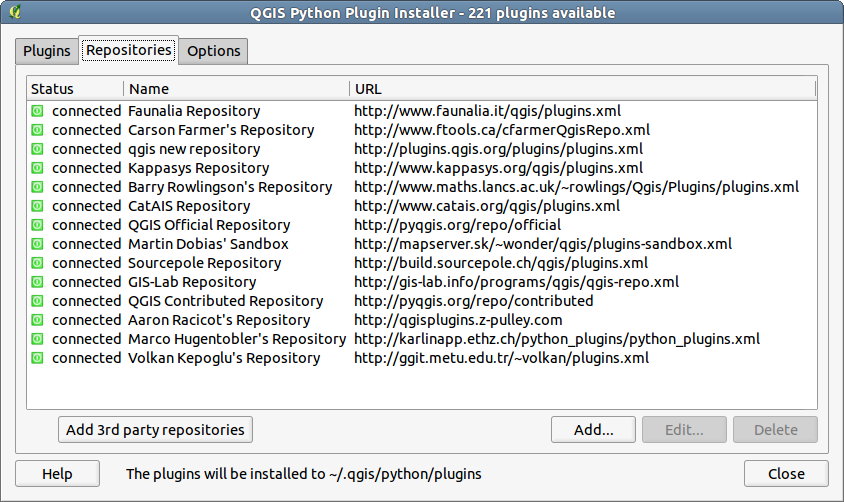
\includegraphics[scale=0.5]{pictures/qgis_plugin/python_installer}
	\caption{QGIS Python Plugin Installer - správa repositářů}
  	\label{pythonplugininstaller}
\end{figure}

QGIS umožňuje uživatelům rozšiřovat funkce programu dle jejich potřeb v podobě zásuvných modulů. Díky dobře zdokumentovanému API může uživatel pohodlně psát pluginy v jazyce C++ nebo Python. Pluginy píší jak vývojáři Quantum GISu, tak i obyčejní uživatelé. Pluginy si můžeme stáhnout z oficiálních či neoficiálních repositářů. Pro instalování pluginů napsaných v jazyce Python a správu repositářů slouží nástroj \textbf{QGIS Python Plugin Installer}, dostupný přes \textit{Plugins $\rightarrow$ Fetch Python Plugins...}.

\noindent Jak je vidět z [\figurename \ref{pythonplugininstaller}], takto nainstalované pluginy se uloží do adresáře: 

\begin{itemize}
	\item \textit{\$HOME$\setminus$.qgis$\setminus$python$\setminus$plugins} - v případě OS GNU/Linux
	\item \textit{C:$\setminus$Documents and Settings$\setminus$USER$\setminus$.qgis$\setminus$python$\setminus$plugins} - v případě OS Windows bývá cesta podobná této.
\end{itemize}

V případě, že uživatel napíše plugin v jazyce Python, doporučuje se ho uložit do výše uvedeného adresáře. Je zde také možnost uložit plugin do adresáře \textit{\$QGIS\_INSTALL\_DIR $\setminus$share$\setminus$qgis$\setminus$python$\setminus$plugins}, ale při případné opětovné kompilaci by byly změny pravděpodobně ztraceny.

\noindent Pluginy psané v jazyce C++ se po přeložení ukládají standardně v \textit{\$QGIS\_INSTALL\_DIR $\setminus$lib$\setminus$qgis$\setminus$plugins}. Uživatel má také možnost nastavit nová úložiště pro svoje pluginy pomocí \textit{Settings $\rightarrow$ Options} a v záložce \textit{Generals} zadat cestu [\figurename \ref{cpprepository}]. \\

\begin{figure}[h]
	\centering
	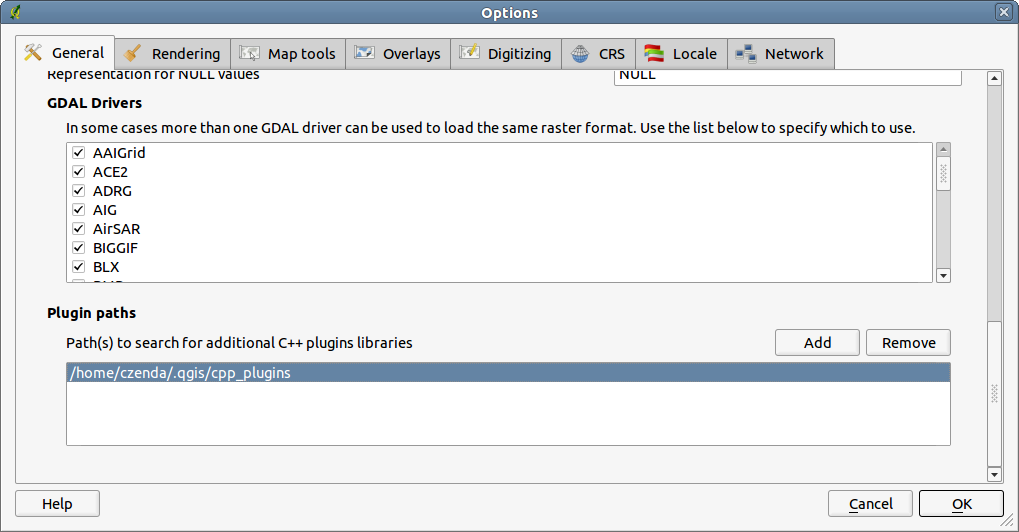
\includegraphics[scale=0.5]{pictures/qgis_plugin/options_cpp_path}
	\caption{\textit{Settings$\rightarrow$Options$\rightarrow$Generals} - přidání nové cesty k pluginům psaných v jazyce C++}
  	\label{cpprepository}
\end{figure}

Všechny nainstalované pluginy, ať psané v jazyce C++ či Python, může uživatel spravovat přes \textbf{QGIS Plugin Manager} - \textit{Plugins$\rightarrow$Manage Plugins...} [\figurename \ref{plugin_manager}].

\begin{figure}[h]
	\centering
	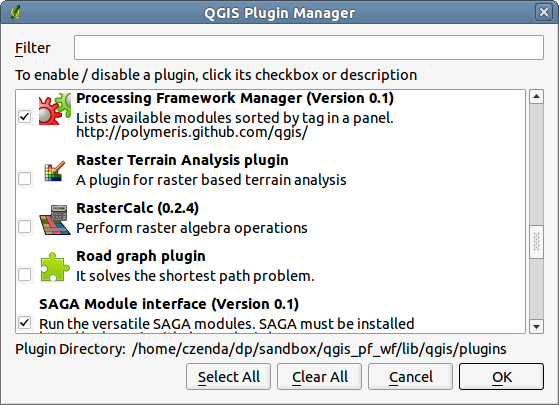
\includegraphics[scale=0.5]{pictures/qgis_plugin/plugin_manager}
	\caption{\textit{Plugins $\rightarrow$Manage Plugins...} - správa pluginů}
  	\label{plugin_manager}
\end{figure}

%%%%%%%%%%%%%%%%%%%%%%%%%%%%%
%% Psaní vlastního pluginu %%
%%%%%%%%%%%%%%%%%%%%%%%%%%%%%
\subsection{Psaní vlastního pluginu}
Pluginy mohou být psány v jazyce C++ a Python. Již z charakteristiky daných jazyků vyplývá, že pro jednoduché, nenáročné či na začátku vývoje pluginu, se bude hodit spíše jazyk Python, který se nemusí kompilovat a píše se v něm rychleji než v~jazyce C++. Pro rozsáhlejší projekty je lepší použít jazyk C++, protože obecně jsou programy psané v kompilovaných jazycích mnohem rychlejší než programy psané v~jazycích interpretovaných. 

%%%%%%%%%%%%
%% Python %%
%%%%%%%%%%%%
\subsection{Python plugin}
\nocite{pyqgis:www}
\index{PyQGIS}
Chceme-li psát plugin v Pythonu, budeme k tomu potřebovat mít nainstalovaný \textbf{QGIS}, \textbf{Python} minimálně verze 2.5, \textbf{Qt} a její pythoní verzi \textbf{PyQt}. Při psaní pluginu v jazyce Python využíváme nástroje PyQGIS. Kromě dokumentace k QGIS API \cite{qgis_api:www} také doporučuji kuchařku, kde nalezneme, jak psát pomocí PyQGIS \cite{pyqgis:www}. Nejjednodušší možnost jak začít psát svůj plugin se jeví využít nástroj \textbf{Plugin Builder}. \textbf{Plugin Builder} je plugin, který vygeneruje základní soubory s kódem. Ty potom můžeme začít upravovat. \\

\noindent Základní soubory jsou:
\begin{itemize}
	\item \textit{\_\_init\_\_.py} - inicializační soubor
	\item \textit{plugin.py} - hlavní soubor pluginu
\end{itemize}

Tyto dva výše zmíněné soubory jsou dostačující k tomu, aby se náš plugin objevil v~\textbf{Plugin Manager}u. Dále budeme potřebovat nějaké grafické rozhraní pro náš plugin. Daný soubor (.ui soubor) si můžeme vytvořit pomocí \textbf{Qt Designer}u a přeložit jej pomocí nástroje \index{pyuic4} \textbf{pyuic4} do souboru Pythonem dobře čitelného. Bude-li náš plugin obsahovat další soubory jako ikony, obrázky či zvuky, vytvoříme si soubor s příponou \textit{.qrc}. Soubor je .xml dokumentem a obsahuje relativní cesty k našim souborům. \textit{.qrc} soubor můžeme vytvořit ručně nebo pomocí \textbf{Qt Designer}u. Soubor poté opět přeložíme do souboru čitelného Pythonem pomocí \index{pyrcc4} \textbf{pyrcc4}.

Pakliže napíšeme plugin, o kterém si myslíme, že by mohl být užitečný, že by ho mohl používat také někdo další, můžeme se pokusit jej nahrát do repositáře. Více informací \url{http://plugins.qgis.org/plugins/} a \url{http://plugins.qgis.org/}.

\subsubsection*{\textit{\_\_init\_\_.py}}
Inicializační soubor, který slouží k získání informací o zásuvném modulu a jeho načtení. Soubor by měl obsahovat funkce $name$(), $description$(), $version$(),\newline $qgisMinimumVersion$() a $authorName$(), které vrací textové řetězce udávající jméno, popis, verzi pluginu, minimální požadovanou verzi QGIS a jméno autora pluginu, a $classFactory$(\textit{iface}).

Funkce $classFactory$(\textit{iface}) vrací instanci třídy reprezentující náš plugin. \textit{iface} odkazuje na instanci třídy \textbf{QgisInterface}, umožňující pluginu přistupovat k funkcím QGIS. Tato funkce je volaná \textbf{QGIS Plugin Manager}em.

Od verze QGIS 2.0 pravděpodobně nebudou akceptována metadata z inicializačního souboru \textit{\_\_init\_\_.py}, ale pouze ze souboru \textit{metadata.txt}.

Ve verzi QGIS 1.9.90 mohou být pluginy zobrazovány nejen v menu \textit{Plugins}, ale mohou být rozděleny pomocí kategorií \textit{Raster}, \textit{Vector}, \textit{Database} a \textit{Web}. V inicializačním souboru tedy přibude funkce $category$(), která tuto informací vrací.

Inicializační soubor může poté vypadat takto [\autoref{plugin:init}]. \\

\begin{lstlisting}[caption={\_\_init\_\_.py - inicializační soubor},label=plugin:init]
def name():
  return "Nazev zasuvneho pluginu"

def description():
  return "Popis pluginu."

def version():
  return "Version 0.1"

def qgisMinimumVersion():
  return "1.0"

def authorName():
  return "Tonda"

def category():
  return "Raster"

def classFactory(iface):
  from plugin import Plugin
  return Plugin(iface)
\end{lstlisting}

\subsubsection*{\textit{plugin.py}}
V souboru \textit{plugin.py} se nachází hlavní třída reprezentující náš plugin. Ta musí obsahovat metody \textit{\_\_init\_\_}, \textit{initGUI} a \textit{unload}. Metoda \textit{\_\_init\_\_} slouží mimo jiné k uchovávání odkazu na \textbf{QgisInterface}. Metoda \textit{initGUI} inicializuje plugin. Inicializace, i když název k tomu svádí, nemusí být spojena s GUI. Metoda \textit{unload}, jak název napovídá, se stará o akce po deaktivaci pluginu. 

\newpage
Soubor se zásuvným modulem korespondující s předchozím inicializačním souborem [\autoref{plugin:init}] by mohl vypadat takto [\autoref{plugin:plugin}]. \\

\begin{lstlisting}[caption={plugin.py - plugin},label=plugin:plugin]
class Plugin:
    def __init__(self, iface):
        self.iface = iface
    def unload(self):
        print "Plugin Plugin by deaktivovan."
    def initGui(self):
		print "Plugin Plugin byl nacten"
\end{lstlisting}

%%%%%%%%%%%%%%%%
%% C++ plugin %%
%%%%%%%%%%%%%%%%
\subsection{C++ plugin}
QGIS Processing Framework je plugin psaný v jazyce Python, proto se zde nebudu mnoho zmiňovat o pluginech psaných v jazyce C++. Více informací o tvorbě pluginů v C++ můžete najít v QGIS Coding and Compilation Guide\footnote{http://download.osgeo.org/qgis/doc/manual/qgis-1.5.0\_coding-compilation\_guide\_en.pdf}.
% 



